\documentclass[10pt]{beamer}
%%%%%%%%%%%%%%%%%%%%%%%%%%%%%%%%%%%%%%%%%%%%%%%%%%%%%%%%%%%%%%%%%%%%%%%%%%%%%%%%%%%%%%%%%%%%%%%%%%%%%%%%%%%%%%%%%%%%%%%%%%%%%%%%%%%%%%%%%%%%%%%%%%%%%%%%%%%%%%%%%%%%%%%%%%%%%%%%%%%%%%%%%%%%%%%%%%%%%%%%%%%%%%%%%%%%%%%%%%%%%%%%%%%%%%%%%%%%%%%%%%%%%%%%%%%%
\usepackage{amsmath}
\usepackage{mathpazo}
\usepackage{hyperref}
\usepackage{multimedia}
\usepackage{multicol}
\usepackage{epsfig}
\usepackage{curves}
\usepackage{epsfig}
\usepackage{epic}
\usepackage{curves}
\usepackage{amsmath}
\usepackage{amssymb}
\usepackage{setspace}
\usepackage{multicol}
\usepackage{algorithm}
\usepackage{algorithmic}
\usepackage{fix-cm}
\usepackage{graphicx}
\usepackage{hyperref}


\setcounter{MaxMatrixCols}{10}
%TCIDATA{OutputFilter=LATEX.DLL}
%TCIDATA{Version=5.00.0.2606}
%TCIDATA{Codepage=932}
%TCIDATA{<META NAME="SaveForMode" CONTENT="1">}
%TCIDATA{BibliographyScheme=Manual}
%TCIDATA{Created=Friday, November 03, 2006 10:56:24}
%TCIDATA{LastRevised=Thursday, February 19, 2015 11:02:18}
%TCIDATA{<META NAME="GraphicsSave" CONTENT="32">}
%TCIDATA{<META NAME="DocumentShell" CONTENT="Other Documents\SW\Slides - Beamer">}
%TCIDATA{Language=American English}
%TCIDATA{CSTFile=beamer.cst}

\newenvironment{stepenumerate}{\begin{enumerate}[<+->]}{\end{enumerate}}
\newenvironment{stepitemize}{\begin{itemize}[<+->]}{\end{itemize} }
\newenvironment{stepenumeratewithalert}{\begin{enumerate}[<+-| alert@+>]}{\end{enumerate}}
\newenvironment{stepitemizewithalert}{\begin{itemize}[<+-| alert@+>]}{\end{itemize} }
\usetheme{Boadilla}

\usefonttheme{serif}
\setbeamercovered{invisible}


%------------------------------------------------
%	PRESENTATION BASICS
%------------------------------------------------


\title[Curating Local Knowledge]{Curating Local Knowledge}
\subtitle{Experimental Evidence from Small Retailers in Indonesia}


\author[Dalton, R{\"u}schenp{\"o}hler, Uras, and Zia]
{
Patricio S. Dalton\inst{1}\
Julius R{\"u}schenp{\"o}hler\inst{2}
Burak Uras\inst{1}\\and
Bilal Zia\inst{3}
}

\institute[]
{
\inst{1} Tilburg University\\
\bigskip
\inst{2} CEGA, UC Berkeley\\
\bigskip
\inst{3} The World Bank\\
}

\date{March 04, 2021}





\title[Curating Local Knowledge]{Curating Local Knowledge}
\subtitle{Experimental Evidence from Small Retailers in Indonesia}


\author[Dalton, R{\"u}schenp{\"o}hler, Uras, and Zia]
{
Patricio S. Dalton\inst{1}\
Julius R{\"u}schenp{\"o}hler\inst{2}
Burak Uras\inst{1}\\and
Bilal Zia\inst{3}
}

\institute[]
{
\inst{1} Tilburg University\\
\bigskip
\inst{2} CEGA, UC Berkeley\\
\bigskip
\inst{3} The World Bank\\
}

\date{March 04, 2021}


%------------------------------------------------
%	PRESENTATION SLIDES
%------------------------------------------------

\begin{document}

\begin{frame}
\titlepage
\end{frame}

%\begin{frame}
%\frametitle{Overview}
%\tableofcontents[hideallsubsections]
%\end{frame}


%------------------------------------------------
\section{Background}

\begin{frame}
\frametitle{Background}
	\begin{itemize}
	\item Micro \& Small firms (MSEs) main \textbf{source of employment} in the developing world
	\vspace{0.2in}
	\item In \textbf{Indonesia}, MSEs represent 99\% of all firms and 94.5\% of employment 
	\vspace{0.2in}
	\item Understanding the factors fostering efficiency and growth of MSEs is an important research and policy goal
	\end{itemize}
\end{frame}

%------------------------------------------------
\begin{frame}
\frametitle{A Growing Focus on Management}
\begin{itemize}
\item \textbf{Classroom Training}: Field, et al. (2010); Karlan \& Valdivia (2011); Bruhn \& Zia (2013); Drexler, Fischer \& Schoar (2014); McKenzie \& Woodruff (2014, 2017); Bulte et al. (2017); Anderson, Chandy \& Zia (2018); Lafortune et al. (2018)
\vspace{0.2in}
\item \textbf{Consulting}: Bloom, et al. (2013); Karlan et al (2015); Bruhn, Karlan \& Schoar (2019)
\vspace{0.2in}

\item \textbf{Mobilizing Peer Knowledge}:
    \begin{itemize}
    \item Brooks et al. (2018) $\rightarrow$ Local mentors (market information)
    \item Cai \& Szeidl (2018) $\rightarrow$ Business meetings
    \item Abebe et al. (2019) $\rightarrow$ Management experience matching
    \end{itemize}
    \vspace{0.2in}
\end{itemize}
\end{frame}


\begin{frame}
\frametitle{What We Do}
\begin{itemize}
\item Some facts about business practices in firms:
	\begin{itemize}	
	\item Vast heterogeneity in business practices and performance across similar businesses (de Mel, McKenzie \& Woodruff, 2009)
	\item Variation in practices accounts for more than 20\% of variation in productivity within the same firm in the US (Bloom et al, 2019)
	\end{itemize}
\vspace{0.2in}
\pause
\item Research thus far has mostly overlooked this underlying heterogeneity in design and implementation of programs
\vspace{0.2in}
\pause
\item Our idea is to make it \textbf{central} to the research design: 
	\begin{itemize}
	\item Use variation across businesses to identify business practices associated with successful performance
	\item Instead of teaching set courses, provide consulting, or matching; we curate what works from local peers
	\item Test different communication channels and their cost-effectiveness
\end{itemize}
\end{itemize}

\end{frame}

\begin{frame}
\frametitle{Selecting Local Best Practices}
\begin{itemize}
\item Detailed \textcolor[rgb]{0.00,0.07,1.00}{qualitative interviews} with local business peers:
    \begin{itemize}
    \item Understand and codify their practices (record-keeping, financial planning, stocking-up, marketing, and joint decision-making)
    \item Identify implementation norms and beliefs regarding each practice (e.g. whether they are complicated, necessary, etc.)
    \item Document locally relevant tips and rule of thumbs
    \end{itemize}
\vspace{0.2in}
\item Baseline \textcolor[rgb]{0.00,0.07,1.00}{quantitative survey}
    \begin{itemize}
    \item Measure practices and outcomes
    \item Quantitative association of business practices with profits and sales
    \end{itemize}
\end{itemize}
\end{frame}

%
\begin{frame}
\frametitle{How Do We Share this Knowledge?}
		\begin{itemize}
		\item \textbf{Handbook}
			\begin{itemize}
			\item \textcolor[rgb]{0.00,0.07,1.00}{Pure information}: Which practices, how to adopt, and why?\\
            %\item \textbf{Positive Frame}: Retailers who implement [x] report y\% \textbf{higher} sales and z\% \textbf{higher} profits.
            %\item \textbf{Negative Frame}: Retailers who do \textbf{not} implement [x] report y\% \textbf{lower} sales and z\% \textbf{lower} profits.
			\end{itemize}
\bigskip
Supplemented with two types of experiential learning:
\bigskip
		\item \textbf{Movie}
			\begin{itemize}
			\item \textcolor[rgb]{0.00,0.07,1.00}{Psychological and emotional involvement}$\rightarrow$ social learning is possible through \textbf{observing the successful experience of similar others}.
			\item Bernard, et al. (2014); La Ferrara et al. (2012); Chong and La Ferrara (2009); Berg and Zia (2013).\\
			\end{itemize}

\bigskip
		\item \textbf{In-shop Light Assistance}
			\begin{itemize}
			\item \textcolor[rgb]{0.00,0.07,1.00}{Hands-on involvement} $\rightarrow$ social learning is possible through own \textbf{experience, with a small nudge} (Kolb, 1984).
			\end{itemize}
			\vspace{0.05in}
%\bigskip
%			$\rightarrow$ Horse race between role models and business counseling.
		\end{itemize}

\end{frame}


\begin{frame}
\frametitle{Research Questions}
	\begin{itemize}
	%\item \textbf{Local characterization}
	%\vspace{0.05in}
	%	\begin{itemize}
	%	\item Which practices are associated with high profits?
	%	\item How do successful businesses implement them?
	%	\end{itemize}
	%\vspace{0.05in}
	\item \textbf{Adoption}
		\begin{itemize}
		\item Do retailers adopt these practices once peer best practices are aggregated and made common knowledge?
		\item If so, ...
			\begin{itemize}
			\item Does the type of experiential involvement matter?
			\end{itemize}
		\end{itemize}
    \vspace{0.3in}
	\item \textbf{Impact}
		\begin{itemize}
		\item Does firm profitability increase?
		\item If so, what are the channels?
		\end{itemize}
	\end{itemize}
\end{frame}


\begin{frame}
\frametitle{Sample}
\begin{itemize}
\item Listing of 2042 small retail businesses from 29 administrative communities (Kelurahan) in urban Jakarta
\item Selection criteria for firm listing:
	\begin{itemize}
%	\item General willingness to grow
	\item At least 4$m^{2}$ in size
	\item At least two different product categories on offer
	\item At least 30 meters distance to next business in sample $\rightarrow$ to minimize spillovers
	\end{itemize}
\item Random sample of 1301 from the list
\item Randomization to treatment arms stratified by
	\begin{itemize}
	\item Gender
	\item Firm space (4-6$m^2$, 6-10$m^2$, 10 and above $m^2$)
	\item Composite score of business practices above or below median
	\item Kelurahan
	\end{itemize}
\end{itemize}
\end{frame}


\begin{frame}
\frametitle{Experimental Design}
	\begin{itemize}
%    \item \textbf{Same set of business practices} across treatments \\
	\item Three types of information provision:
	\vspace{0.05in}
		\begin{itemize}
		\item \textcolor[rgb]{0.00,0.07,1.00}{Handbook} with best practices and tips
		\vspace{0.05in}
		\item \textcolor[rgb]{0.00,0.07,1.00}{Movie} with successful peers
		\vspace{0.05in}
		\item Business practice implementation \textcolor[rgb]{0.00,0.07,1.00}{assistance}
		\end{itemize}
	\vspace{0.05in}
\end{itemize}
	\begin{itemize}
\item{Five experimental groups}
        %\begin{itemize}
        %\item{Handbooks (N=1040)}
        %: Positive Framing (N=520) and Negative Framing (N=520)}\\
	\vspace{0.05in}
            \begin{enumerate}
              \item \textcolor[rgb]{0.00,0.07,1.00}{Handbook} only (N=260)
              \item \textcolor[rgb]{0.00,0.07,1.00}{Handbook} and invitation to \textcolor[rgb]{0.00,0.07,1.00}{movie} screening (N=260)
              \item \textcolor[rgb]{0.00,0.07,1.00}{Handbook} and offer of two \textcolor[rgb]{0.00,0.07,1.00}{assistance} visits (N=260)
              \item \textcolor[rgb]{0.00,0.07,1.00}{Handbook} and both \textcolor[rgb]{0.00,0.07,1.00}{movie} and \textcolor[rgb]{0.00,0.07,1.00}{assistance} (N=260)
              \item Control (N=261)
            \end{enumerate}
        \end{itemize}
    %\end{itemize}
\end{frame}


\begin{frame}
\frametitle{Timeline}
\begin{enumerate}
    \item September 2015: \textcolor[rgb]{0.00,0.07,1.00}{Qualitative} Interviews
    \item[]
    \item January 2016: \textcolor[rgb]{0.00,0.07,1.00}{Listing} for Baseline
    \item[]
    \item Feb-Apr 2016: \textcolor[rgb]{0.00,0.07,1.00}{Baseline} Survey
    \item[]
    \item Oct-Nov 2016: \textcolor[rgb]{0.00,0.07,1.00}{Interventions}
    \item[]
    \item Apr-May 2017: \textcolor[rgb]{0.00,0.07,1.00}{Midline}
    \item[]
    \item Apr-May 2018: \textcolor[rgb]{0.00,0.07,1.00}{Endline}
\end{enumerate}
\end{frame}


\begin{frame}
\frametitle{Typical Retail Shop in the Sample}

\begin{figure}[htbp]
	\centering
		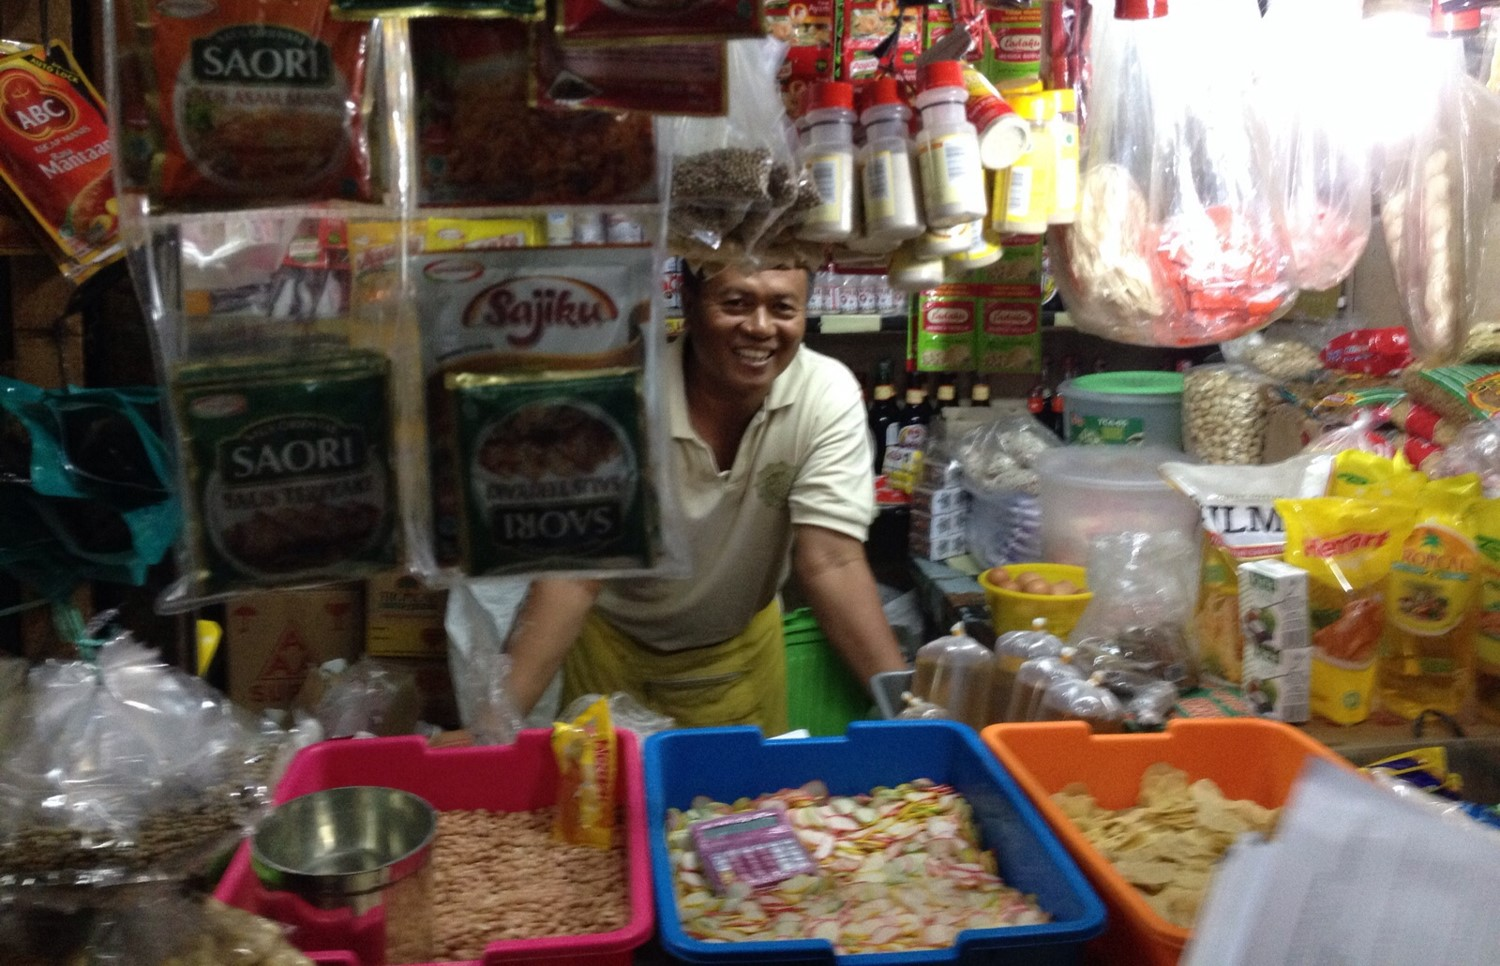
\includegraphics[width=4in]{retailer1.jpg}
	%\caption{Best-practices handbook}
	\label{height}
\end{figure}
\end{frame}

\begin{frame}
\frametitle{Typical Retail Shop in the Sample II}

\begin{figure}[htbp]
	\centering
		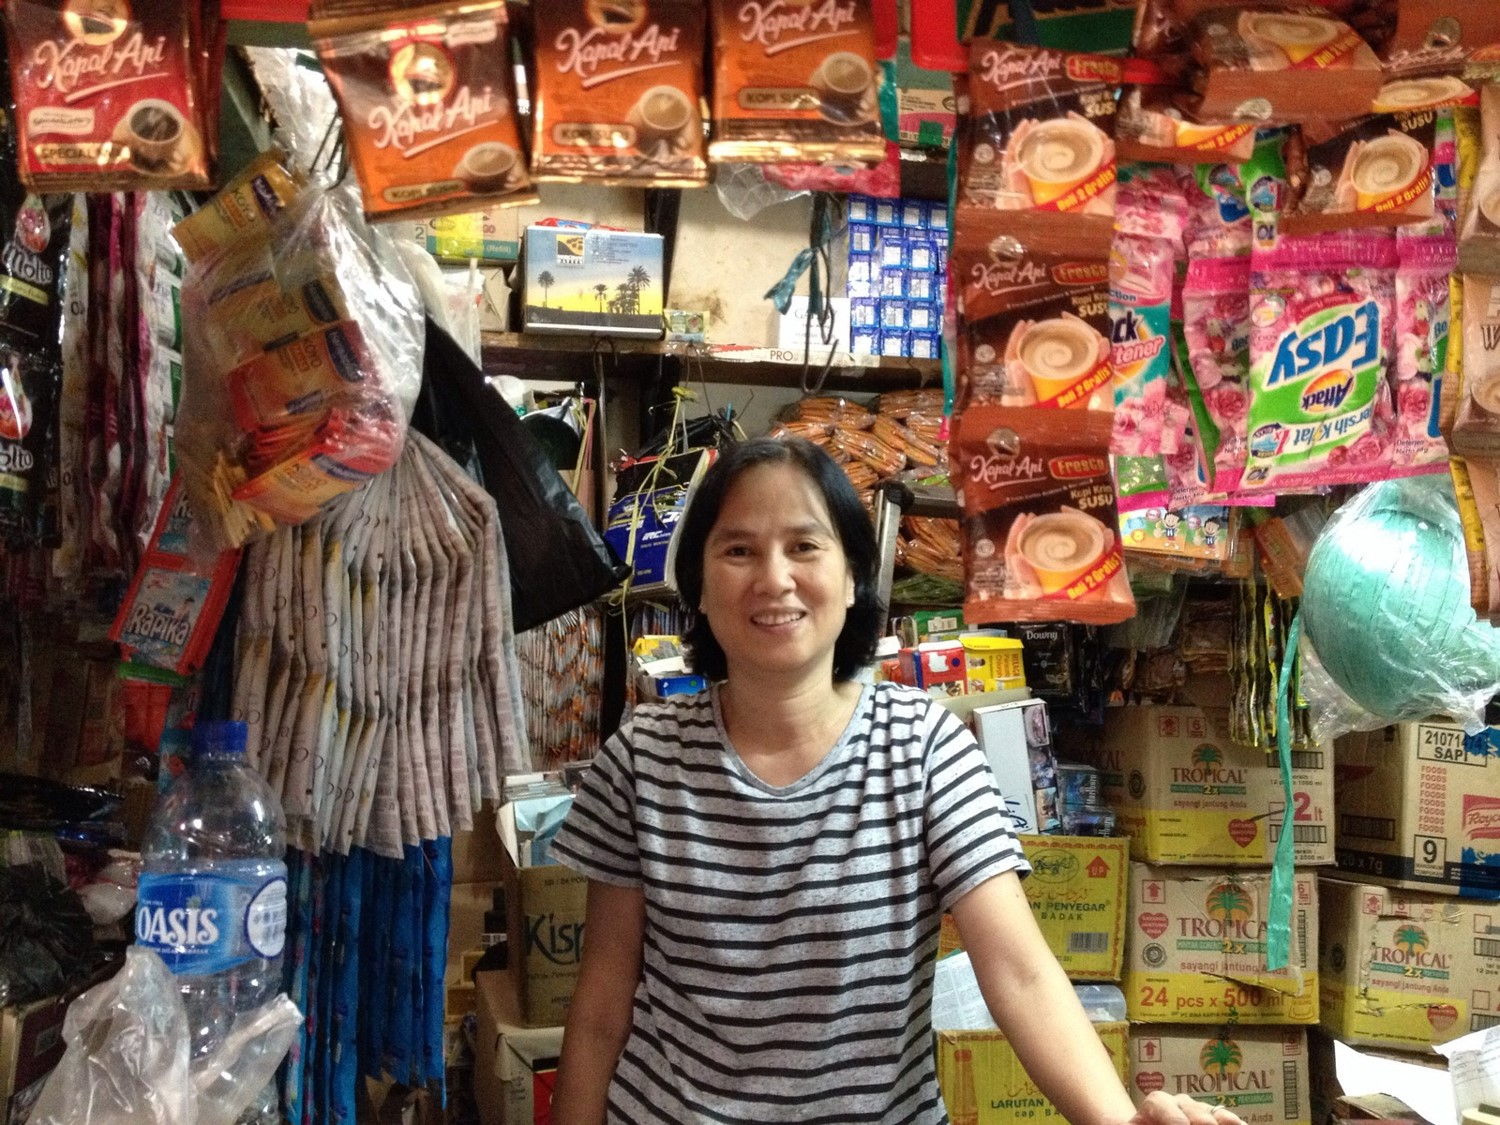
\includegraphics[width=4in]{retailer2.jpg}
	%\caption{Best-practices handbook}
	\label{height}
\end{figure}
\end{frame}


\begin{frame}
\frametitle{Handbook}

\begin{figure}[htbp]
	\centering
		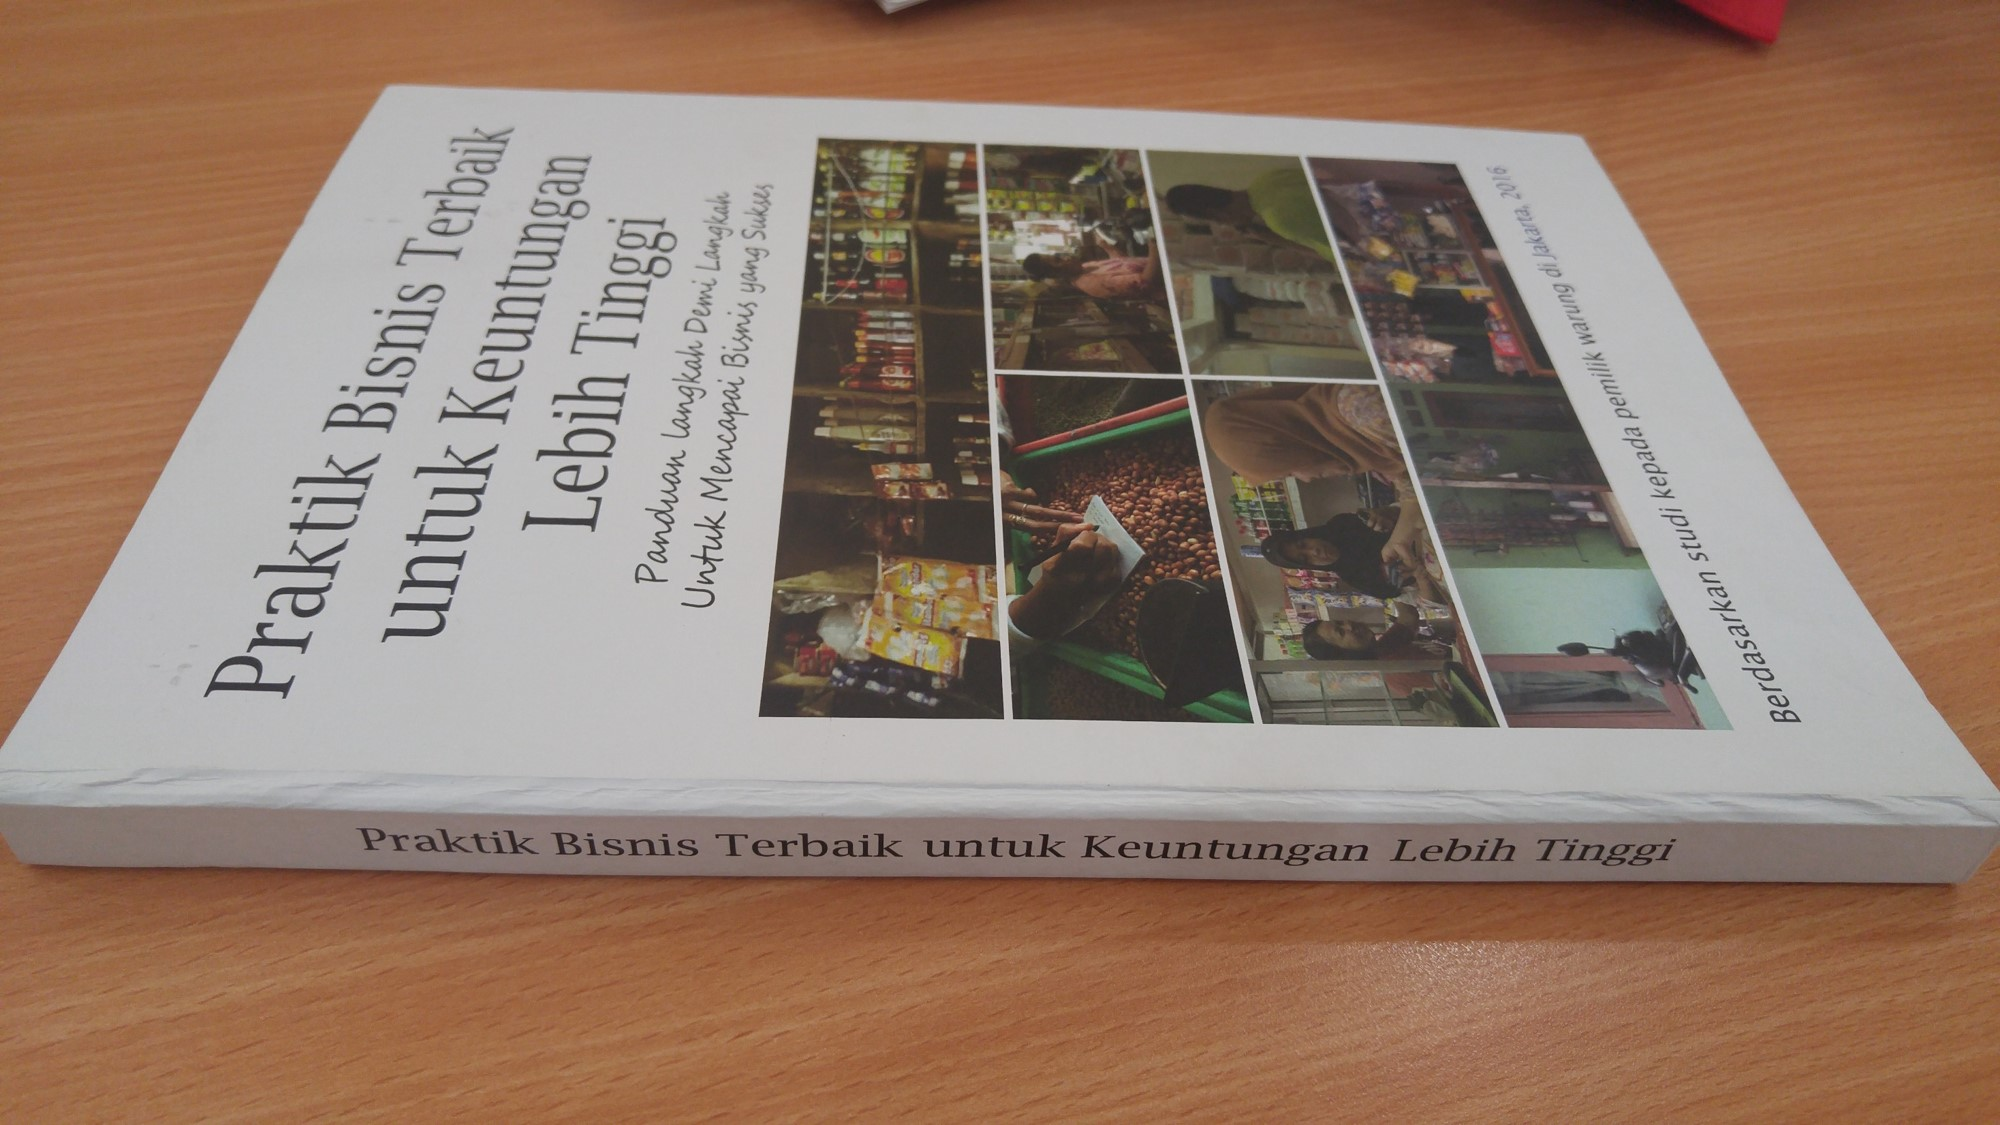
\includegraphics[width=4in]{handbook.jpg}
	
	\label{height}
\end{figure}
\end{frame}


\begin{frame}
\frametitle{Handbook Content}
\begin{figure}[htbp]
	\centering
		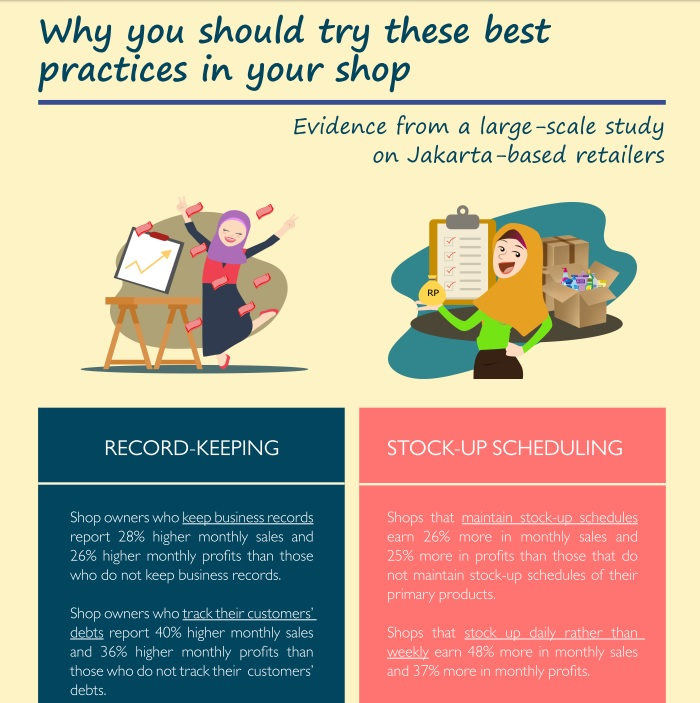
\includegraphics[width=2.6in]{Handbook_return.jpg}
	
	\label{height}
\end{figure}
\end{frame}


\begin{frame}
\frametitle{Handbook Content II}

\begin{figure}[htbp]
	\centering
		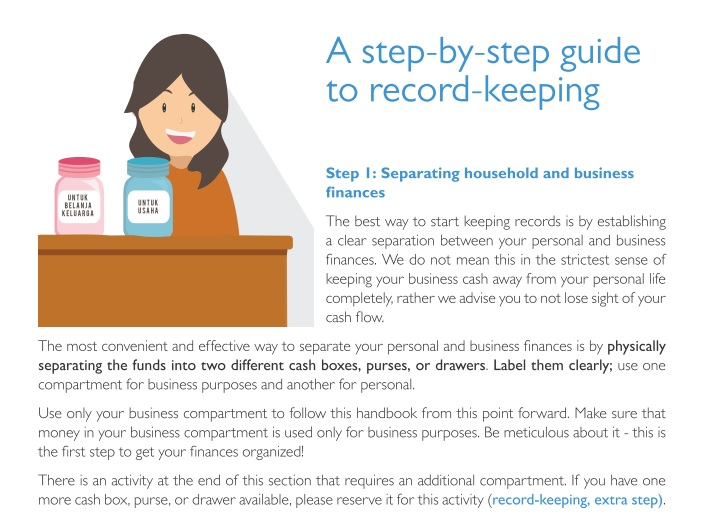
\includegraphics[width=2.6in]{Handbook_stepbystep.jpg}
	
	\label{height}
\end{figure}
\end{frame}

\begin{frame}
\frametitle{Movie with Successful Peers}
\begin{figure}[htbp]
	\centering
		\includegraphics[width=4.4in]{movie.jpg}
   
	\label{height}
\end{figure}
\end{frame}


\begin{frame}
\frametitle{Implementation Assistance for Business Practices}
\begin{figure}[htbp]
	\centering
		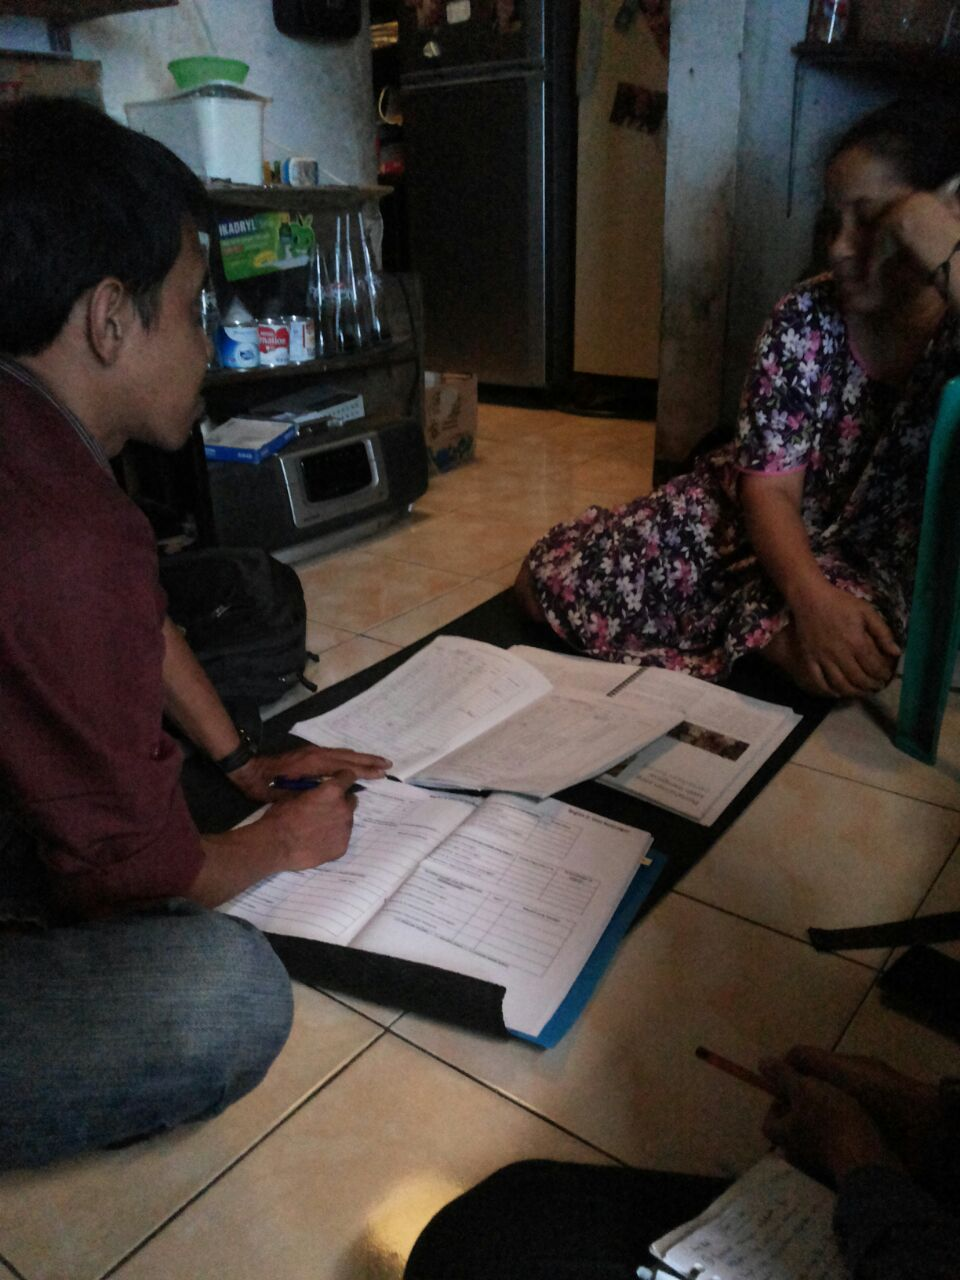
\includegraphics[width=2.0in]{Assistance_expl.jpg}
	
	\label{height}
\end{figure}
\end{frame}


\section{Data and Analysis}


\begin{frame}
\frametitle{Summary Statistics}
{\tiny{
	\begin{table}
		%\begin{adjustbox}{width=9.6cm}
		\centering	
		%\tabcolsep=0.2cm

			\begin{tabular}{l*{10}{c}}
			\hline\hline
			\hline


&\multicolumn{1}{c}{\textbf{Control}}
&&\multicolumn{1}{c}{\textbf{HB only}}	
&&\multicolumn{1}{c}{\textbf{HB \& MOV}	}
&&\multicolumn{1}{c}{\textbf{HB \& HELP}}	
&&\multicolumn{1}{c}{\textbf{HB \& MOV}}	\\


&\multicolumn{1}{c}{}
&&\multicolumn{1}{c}{}	
&&\multicolumn{1}{c}{}
&&\multicolumn{1}{c}{}	
&&\multicolumn{1}{c}{\textbf{\& HELP}}	\\


&\textit{N = 261}	
&&\textit{N = 260}	
&&\textit{N = 260}	
&&\textit{N = 260}	
&&\textit{N = 260}	\\
\hline \\

\textbf{Firm Owner Characteristics} \\
Gender (Male=1)											& 0.28	&& 0.3	&&0.29	&& 0.3	&& 0.28\\
Age														&45.22	&&45.27	&&45.28	&&45.16	&&45.38 \\
Education (Years)										&9.1	&&9.52	&&9.36	&&9.42	&&9.55 \\
%Digitspan												& 1.7	&& 1.67 && 	1.8 &&	1.67	&& 1.69 \\
														%&(1.12) 	&& 		&& 		&& 		&& 		&& \\
Risk Preference (0 - 10 ``Perfectly Risk-Seeking'')		&3.74	&&3.76	&&3.88	&&3.6	&&3.68 \\											
Time Preference	(0 - 10 ``Perfect Patience'')			&5.19	&&5.07	&&5.21	&&5.25	&&5.2 \\[0.5ex]
\\														
\textbf{Firm Characteristics} \\
Firm Age (Years)										&12.76		&&13.77		&&14.03		&&13.98		&&13.47 \\
Family Member Is Business Partner							&0.56		&&0.6		&&0.63		&&0.59		&&0.62 \\
Total Number of Workers									&2.03		&&2.05		&&1.9		&&1.99		&&2.04 \\
%Number of Full Time Paid Employees						&0.09		&&0.1		&&0.08		&&0.08		&&0.11		&&0.08 \\
														%&(0.3)		&&			&&			&&			&&			&& \\
Business Has Tax ID										&0.2		&&0.21		&&0.2		&&0.15		&&0.18 \\
Total Sales Last Month (USD PPP)						&4454.37 &&	4730.64	&& 4840.55	&& 4761.4	&& 5139 \\
												
Total Profits Last Month (USD PPP)						& 889.58	&& 961.1 &&	926.78	&& 825.25	&& 934.66 \\
Applied for Bus Loan in Last 12 Months
			    & 0.2	&& 0.17	&& 0.15	&& 0.22	&& 0.17 \\
													
Obtained Bus Loan in Last 12 Months
						& 0.18 &&	0.15	&& 0.14	&& 0.18	&& 0.14 \\[0.5ex]
\\
\\
\textbf{Business Practices} \\
Management Practices Aggregate Score											& 0.37	&& 0.36	&& 0.37	&& 0.35	&& 0.37 \\
\hspace{3mm}Marketing Subscore												& 0.23	&& 0.23 &&	0.25	&& 0.23	&& 0.24 \\
\hspace{3mm}Stocking-up	Subscore											& 0.45	&& 0.47	&& 0.47	&& 0.47	&& 0.46 \\
\hspace{3mm}Record-keeping Subscore											& 0.33	&& 0.28	&& 0.3	&& 0.29 &&	0.3 \\
\hspace{3mm}Financial-planning Subscore									& 0.51	&& 0.47	&& 0.47	&& 0.43	&& 0.47 \\
%\hspace{3mm} Discussion Subscore                        & 0.57	&& 0.59	  && 0.61	&& 0.6	&& 0.64  \\
&		&&		&&		&& \\
		\hline
		\hline
			\end{tabular}
		%\end{adjustbox}			
		
		%\begin{adjustbox}{center}
			%\begin{tabular}{l*{12}{l}}
			%\multicolumn{13}{p{0.95\textwidth}}{\footnotesize \textit{Notes}: $^1$ Last month's sales and profits appear with both tails winsorized at 1%.}
			%\end{tabular}
		%\end{adjustbox}	
		
	\end{table}}}
\begin{itemize}
\item Test of Joint Orthoganality from Multinomial Logit (P-value): 0.857
\end{itemize}
\end{frame}


\begin{frame}
\frametitle{Movie: Take Up and Assessment}
{\scriptsize{\begin{table}[htbp]
%\fontsize{10}{11}\selectfont
  \centering
 %   \tabcolsep=0.10cm
    %\begin{adjustbox}{width=11cm}
    \begin{tabular}{lcc}
    \hline
   	& (1)   					&(2)   						 \\
    \hline
  	& \textbf{HB \& MOV} 		& \textbf{HB \& MOV}		  \\
  	& 							& \textbf{\& HELP}			\\
   	& \textbf{(A)}   			& \textbf{(B)}   			 \\
 	&							&							\\
% 	&							&							&& \textit{F-test}\\
   	%	& Assigned 				& Assigned 					&&  \\
   	& \textit{N=260} 			& \textit{N=260} 			 \\
   \hline
   														&		&		 \\
    \textbf{Attendance} 								&       &         \\
  	% 													&		&		&& \\
    Business Owner or Partner Attended Film Screening 	& 0.52  & 0.49   \\
    %Baseline respondent attended film screening 		& 0.47  & 0.45  && 0.792 \\
   	%Respondent was reminded by phone 					& 0.05  & 0.07  && 0.355 \\
    %Respondent was reminded by visit to business 		& 0.35  & 0.33  && 0.782 \\
    %Distance to screening location (in decimal degrees)& 0.01  & 0.01  && 0.869 \\
	&       &       \\
    \textbf{Evaluation (1-4 Scale):}	&       &        \\
   	%									&       &       &&  \\
    Has Learned Something New	& 3.34  & 3.21  \\
    Feels Inspired 				& 3.31  & 3.30   \\
    Feels Hopeful 				& 3.60  & 3.42   \\
    Feels Bored 				& 0.83  & 0.97    \\
    \end{tabular}
   % \end{adjustbox}

\end{table}}}

\end{frame}


%%% Attendance and feedback to assistance + comparison between experimental groups
\begin{frame}

\frametitle{Assistance: Take Up and Assessment}
{\scriptsize{\begin{table}[htbp]
%\fontsize{10}{11}\selectfont
  \centering
    %\tabcolsep=0.10cm
   % \begin{adjustbox}{width=11cm}
    \begin{tabular}{lcc}
    \hline
    & (1)   			& (2) 			\\
    \hline
   	& \textbf{HB \& HELP} 		& \textbf{HB \& MOV,}		 \\
  	& 							& \textbf{\& HELP}			 \\
   	& \textbf{(A)}   			& \textbf{(B)}   			\\
	&							&							 \\
% 	&							&							&& \textit{F-test}\\
   	%	&& Assigned 				& Assigned 					&&  \\
   	& \textit{N=260} 			& \textit{N=260} 		\\
    \hline
          																				&       &      \\
    \multicolumn{1}{l}{\textbf{Attendance}} 											&       &        \\
    %\multicolumn{1}{l}{\textit{1st session}} 											&       &       & &  \\
    \multicolumn{1}{l}{    Business Owner or Partner Attended 1st Session} 				& 0.77  & 0.78  \\
    %\multicolumn{1}{l}{    Baseline respondent attended 1st session} 					& 0.76  & 0.77  && 0.756 \\
    %\multicolumn{1}{l}{    Recipient plans to use at least one new practice} 			& 0.37  & 0.47  && 0.021** \\
    %\multicolumn{1}{l}{    Recipient plans neither handbook study nor implementation} 	& 0.12  & 0.11  && 0.784 \\
         														 						%&     	&       &&  \\
    %\multicolumn{1}{l}{\textit{2nd session}} 											&       &       &&  \\
    \multicolumn{1}{l}{    Business Owner or Partner Attended 2nd Session} 				& 0.68  & 0.68   \\
    %\multicolumn{1}{l}{    Baseline respondent attended 2nd session} 					& 0.67  & 0.67  && 1 \\
    %\multicolumn{1}{l}{    Recipient plans to use at least one new practice} 			& 0.39  & 0.47  && 0.063* \\
    %\multicolumn{1}{l}{    Recipient plans neither handbook study nor implementation} 	& 0.13  & 0.08  && 0.044** \\
          																				&       &        \\
    \multicolumn{1}{l}{\textbf{Evaluation (1-4 Scale)}} 								&       &         \\
    \multicolumn{1}{l}{Has Learned Something New} 										& 2.88  & 2.89   \\
    \multicolumn{1}{l}{Feels Inspired} 													& 2.76  & 2.83   \\
    \multicolumn{1}{l}{Feels Hopeful} 													& 2.88  & 2.97  \\
    \multicolumn{1}{l}{Feels Bored} 													& 0.59  & 0.43   \\
    \end{tabular}
   % \end{adjustbox}

\end{table}}}
\end{frame}


\begin{frame}
\frametitle{Impact on Business Practices}
\framesubtitle{Aggregate Scores}
{\tiny{\begin{table}[t]
%\centering
%\begin{adjustbox}{width=10cm}
%	\tabcolsep=0.05cm
	\begin{tabular}{l*{10}{c}}
		\hline \hline
		\\
			&\textbf{Record}			&&\textbf{Planning}			&&\textbf{Stocking-up}	&&\textbf{Marketing} && \textbf{Joint} \\
&\textbf{Keeping}                       &&                        &&	                   &&	 && Decision-making \\
					&(1)					&&(2)						&&(3) 						&&(4) && (5)\\
			\cline{2-2}					\cline{4-4}					\cline{6-6}			\cline{8-8} \cline{10-10}  \\


Assigned Handbook 			&                    0.025   &&	          0.027   	 &&           -0.007   	 &&          -0.011   	  &&         0.011
      \\
         							&               (0.209)   	   &&      (0.273)   	&&         (0.694)   	     &&    (0.694)   	&&         (0.694)
    \\

         							
Assigned Handbook \& Movie 	&                     0.057*** 	 &&          0.043  	   &&       0.038  	    &&       0.040    &&        0.040        \\
          							&              (0.009)   &&	         (0.107)   	  &&       (0.117)   	  &&       (0.166)   	 &&        (0.217)         \\

         							
Assigned Handbook \& Assistance 	&              0.065*** 	  &&         0.034   	&&           0.011   	 &&           0.039 	       &&      0.037    \\
         							&           (0.004)   	  &&       (0.166)   &&	         (0.664)   && 	         (0.166)   	  &&       (0.239)    \\

         							
Assigned All Three          	&                0.054***	  &&         0.068***  	 &&          0.053**  	    &&       0.061**	   &&        0.059*          \\
									&             (0.009)    &&	         (0.009)   	&&         (0.020)   	  &&       (0.032)   &&	         (0.094)           \\

\hline         							
\\
R-squared									&               0.204   	 &&          0.192   	&&           0.187   	&&           0.150	 &&           0.120             \\
Sample Size 								&               2205   	  &&          2204   	   &&         2205   	 &&           2205   	    &&        2205      \\
Dependent Variable Mean of Control 		&                  0.196  	  &&         0.402   	 &&          0.471    &&	           0.250    	 &&          0.269          \\
Dependent Variable SD of Control 			&              0.252    	 &&          0.310   	  &&         0.270      	  &&         0.320    && 	           0.420        	\\
F-tests (p-value):							&			&&			&&			&&			\\
\hspace{5mm}Book = Book \& Mov				        &               0.069   	   &&           0.487   	  &&          0.014     	  &&          0.028    	 &&          0.300           \\
\hspace{5mm}Book = Book \& Assistance				        &               0.025  	  &&          0.754     	 &&           0.304   	 &&          0.030    	  &&          0.348                 \\
\hspace{5mm}Book = All Three				        &                  0.096    	  &&         0.073    	    &&      0.001   	  &&         0.002    &&	         0.082        \\
\hline
	\end{tabular}
%\end{adjustbox}
\end{table}}}
\begin{itemize}
\item Multiple hypothesis testing corrected p-values in parentheses
\item "All Three" improvement of 28 \% in record-keeping, 17 \% in planning, 11 \% in stocking, 24 \% in marketing and 22 \% in joint decision making.
\end{itemize}
\end{frame}


\begin{frame}

\frametitle{\centering{Business Profits}}
{\scriptsize{\begin{table}[t]
\centering
%\begin{adjustbox}{width=9cm}
%	\tabcolsep=0.05cm
	\begin{tabular}{l*{5}{c}}
\hline
\hline
			   &&Profits	        &&Profits \\
				&&last month  		&&last month \\
			&&(win 5\%)			&&(IHS) \\
				&&(1)				&&(2)	\\
&& \\
					\hline
&&\\
		

Assigned Handbook 					&&-91.307   	&& -0.067   		\\
       								 	&&         (78.400)  	&&          (0.088)  	\\

         							
Assigned Handbook \& Movie				&&110.378   	  	&& 0.055   		\\
       									&&         (86.841)  	&&          (0.092)  	\\

         							
Assigned Handbook \& Assistance 	&&         310.455***	&&           0.261***		\\
       								 	&&         (89.488) 	&&          (0.096)  	\\
         							
Assigned All Three          		&&         191.088**  	&&           0.199** 		\\
       								 	&&         (84.662)  	&&          (0.094)  	\\

   	\\
\hline         							
\\
R-squared											  	&& 0.179  	&& 0.211  	\\
Sample Size 											&&2172	&& 2172 	\\
Dependent Variable Mean in Control Group			 	&&          894.544   	&&           6.817 	\\
Dependent Variable SD in Control Group				 	&&         1127.783   	 &&          1.348  	\\
F-tests (p-value):											&&			&&			\\
\hspace{5mm}Book = Book \& Mov				        	&&    0.020   	&&            0.167 	\\
\hspace{5mm}Book = Book \& Assistance				  			&&0.000   	&&0.000  	\\
\hspace{5mm}Book = All Three			   			  	&&0.001   	&&0.003  	\\
\hline
	\end{tabular}
%\end{adjustbox}

\end{table}}}
\begin{itemize}
\item Profits increase by 35\% (about 0.28 sd.) - ITT.
\end{itemize}
\end{frame}




\begin{frame}
\frametitle{Business Sales}
{\scriptsize{\begin{table}[t]
\centering
%\begin{adjustbox}{width=9cm}
%	\tabcolsep=0.05cm
	\begin{tabular}{l*{5}{c}}
\hline
\hline
                &&ITT	        &&TOT \\
			   &&Sales	        &&Sales \\
				&&last month  		&&last month \\
			&&(win 5\%)			&&(win 5\% \\
				&&(1)				&&(2)	\\
&& \\
					\hline
&&\\
		

Assigned Handbook 					&&-396.976   	&&               -417.198		\\
       								 	&&        (314.252)   	&&          -417.198	\\

         							
Assigned Handbook \& Movie				&&335.489   	  	&& 601.221    		\\
       									&&       (337.881)  	&&            (606.634)	\\

         							
Assigned Handbook \& Assistance 	&&                   836.755**	&&                     1031.692** 	\\
       								 	&&        (372.924) 	&&            (457.015) 	\\
         							
Assigned All Three         		&&         807.462**  	&&                         1558.326**		\\
       								 	&&        (358.384)  	&&          (696.317)   	\\

   	\\
\hline         							
\\
R-squared											  	&& 0.492  	&&  0.483	\\
Sample Size 											&& 2197	&& 2197 	\\
Dependent Variable Mean in Control Group			 	&&         4998.923   &&	          4998.923 	\\
Dependent Variable SD in Control Group				 	&&         5623.257   	&&           5623.257	\\
F-tests (p-value):											&&			&&			\\
\hspace{5mm}Book = Book \& Mov				        	&&            0.020 	&&           0.047 	\\
\hspace{5mm}Book = Book \& Assistance				  			&&0.000   	&& 0.000 	\\
\hspace{5mm}Book = All Three			   			  	&&0.000   	&&0.001  	\\
\hline
	\end{tabular}
%\end{adjustbox}

\end{table}}}
\begin{itemize}
\item Sales increase by 16\% (about 0.15 sd.) - ITT %- and 31\% (0.28 sd.) - TOT.
\end{itemize}
\end{frame}


\begin{frame}
\frametitle{Other Outcomes}
\begin{itemize}
\item \textbf{No significant} impacts on:
    \begin{itemize}
    \vspace{0.2in}
    \item Business expenses
    \vspace{0.2in} 		
    \item Size of the shop
      \vspace{0.2in}
    \item Number of employees
      \vspace{0.2in}
    \item Number of customers
       \vspace{0.2in}
     \item Business credit
    \end{itemize}
\end{itemize}
\end{frame}


\begin{frame}
\frametitle{Efficiency Gains?}
\begin{enumerate}
\item Unpacking impacts on practices shows improvements in efficiency practices:
\vspace{0.1in}
\begin{itemize}
\item Adjust stocks based on product profitability
\item Negotiate lower prices with suppliers
\item Consult with former customers
\item Offer discounts
\item Make joint decisions
\item Review financial performance to identify channels of improvement
\item Make anticipated budget for upcoming costs
\end{itemize}
\vspace{0.2in}
\pause
\item These are non-record-keeping practices. Also, variance in profits among the treated businesses does not converge
\vspace{0.2in}
\pause
\item Causal-mediation analysis shows that the most important drivers of impact on sales and profits are stocking up and marketing practices.
\end{enumerate}
\vspace{0.2in}
$\rightarrow$ \textcolor[rgb]{0.00,0.07,1.00}{Efficiency gains}
\end{frame}

\begin{frame}
\frametitle{Knowledge or Aspirations?}
\begin{itemize}
\item Our interventions could have increased business performance and practice adoption through an increase in business aspirations rather than (or on top of) business knowledge.
\vspace{0.2in}
\item We directly measure business aspirations at baseline, midline, and endline for all shop owners in the sample.
\vspace{0.2in}
\item We elicit short (one year) and long-term (ideal) aspirations on various business dimensions:
\vspace{0.1in}
    \begin{itemize}
    \item sales
    \item shop size
    \item number of customers
    \item number of employees
    \end{itemize}
\vspace{0.2in}
\item No treatment effects on aspirations
\vspace{0.2in}
\end{itemize}
$\rightarrow$ \textcolor[rgb]{0.00,0.07,1.00}{Knowledge}
\end{frame}

\begin{frame}
\frametitle{Business Stealing?}
Do treated businesses improve performance at the expense of the control group?
\vspace{0.1in}
\begin{itemize}
\item Shops in Control group \textbf{do not decrease} their sales and profits from baseline to endline. They remain the same.
\vspace{0.1in}
\item Shops in Control group that are closer to the treated shops \textbf{do not suffer bigger losses in sales and profits} than those who are further away.
\end{itemize}
\vspace{0.2in}
$\rightarrow$ \textcolor[rgb]{0.00,0.07,1.00}{No evidence for business stealing}
\end{frame}

\begin{frame}
\frametitle{Cost-Effectiveness}
\begin{itemize}
\item \textbf{Low cost} per firm:
\begin{itemize}
\item Cost Handbook alone: USD 100
\item Cost Handbook \& Movie: USD 125
\item Cost Handbook \& Assistance: USD 125
\item Cost Handbook \& Assistance \& Movie: USD 150
\vspace{0.20in}
\end{itemize}
\item \textbf{High Benefits}
    \begin{itemize}
    \item Up to USD 330 per month in profits.
    \item Adoption of top practices by retailers.
    \end{itemize}
\vspace{0.20in}
 \item Research Design \textbf{scalable and replicable} in other settings.
\end{itemize}
\end{frame}


%--------------------------------------
\begin{frame}
\frametitle{Takeaways}
\begin{itemize}
    \item Curating local knowledge has value for business growth 
            \vspace{0.20in}
    \item Knowledge alone does not have an impact but needs additional help or nudges
            \vspace{0.20in}
	\item These "add-ons" are inexpensive and scalable, making this type of intervention very attractive for policy
    
\end{itemize}
\end{frame}


\end{document}
